\begin{figure}[t] \centering 
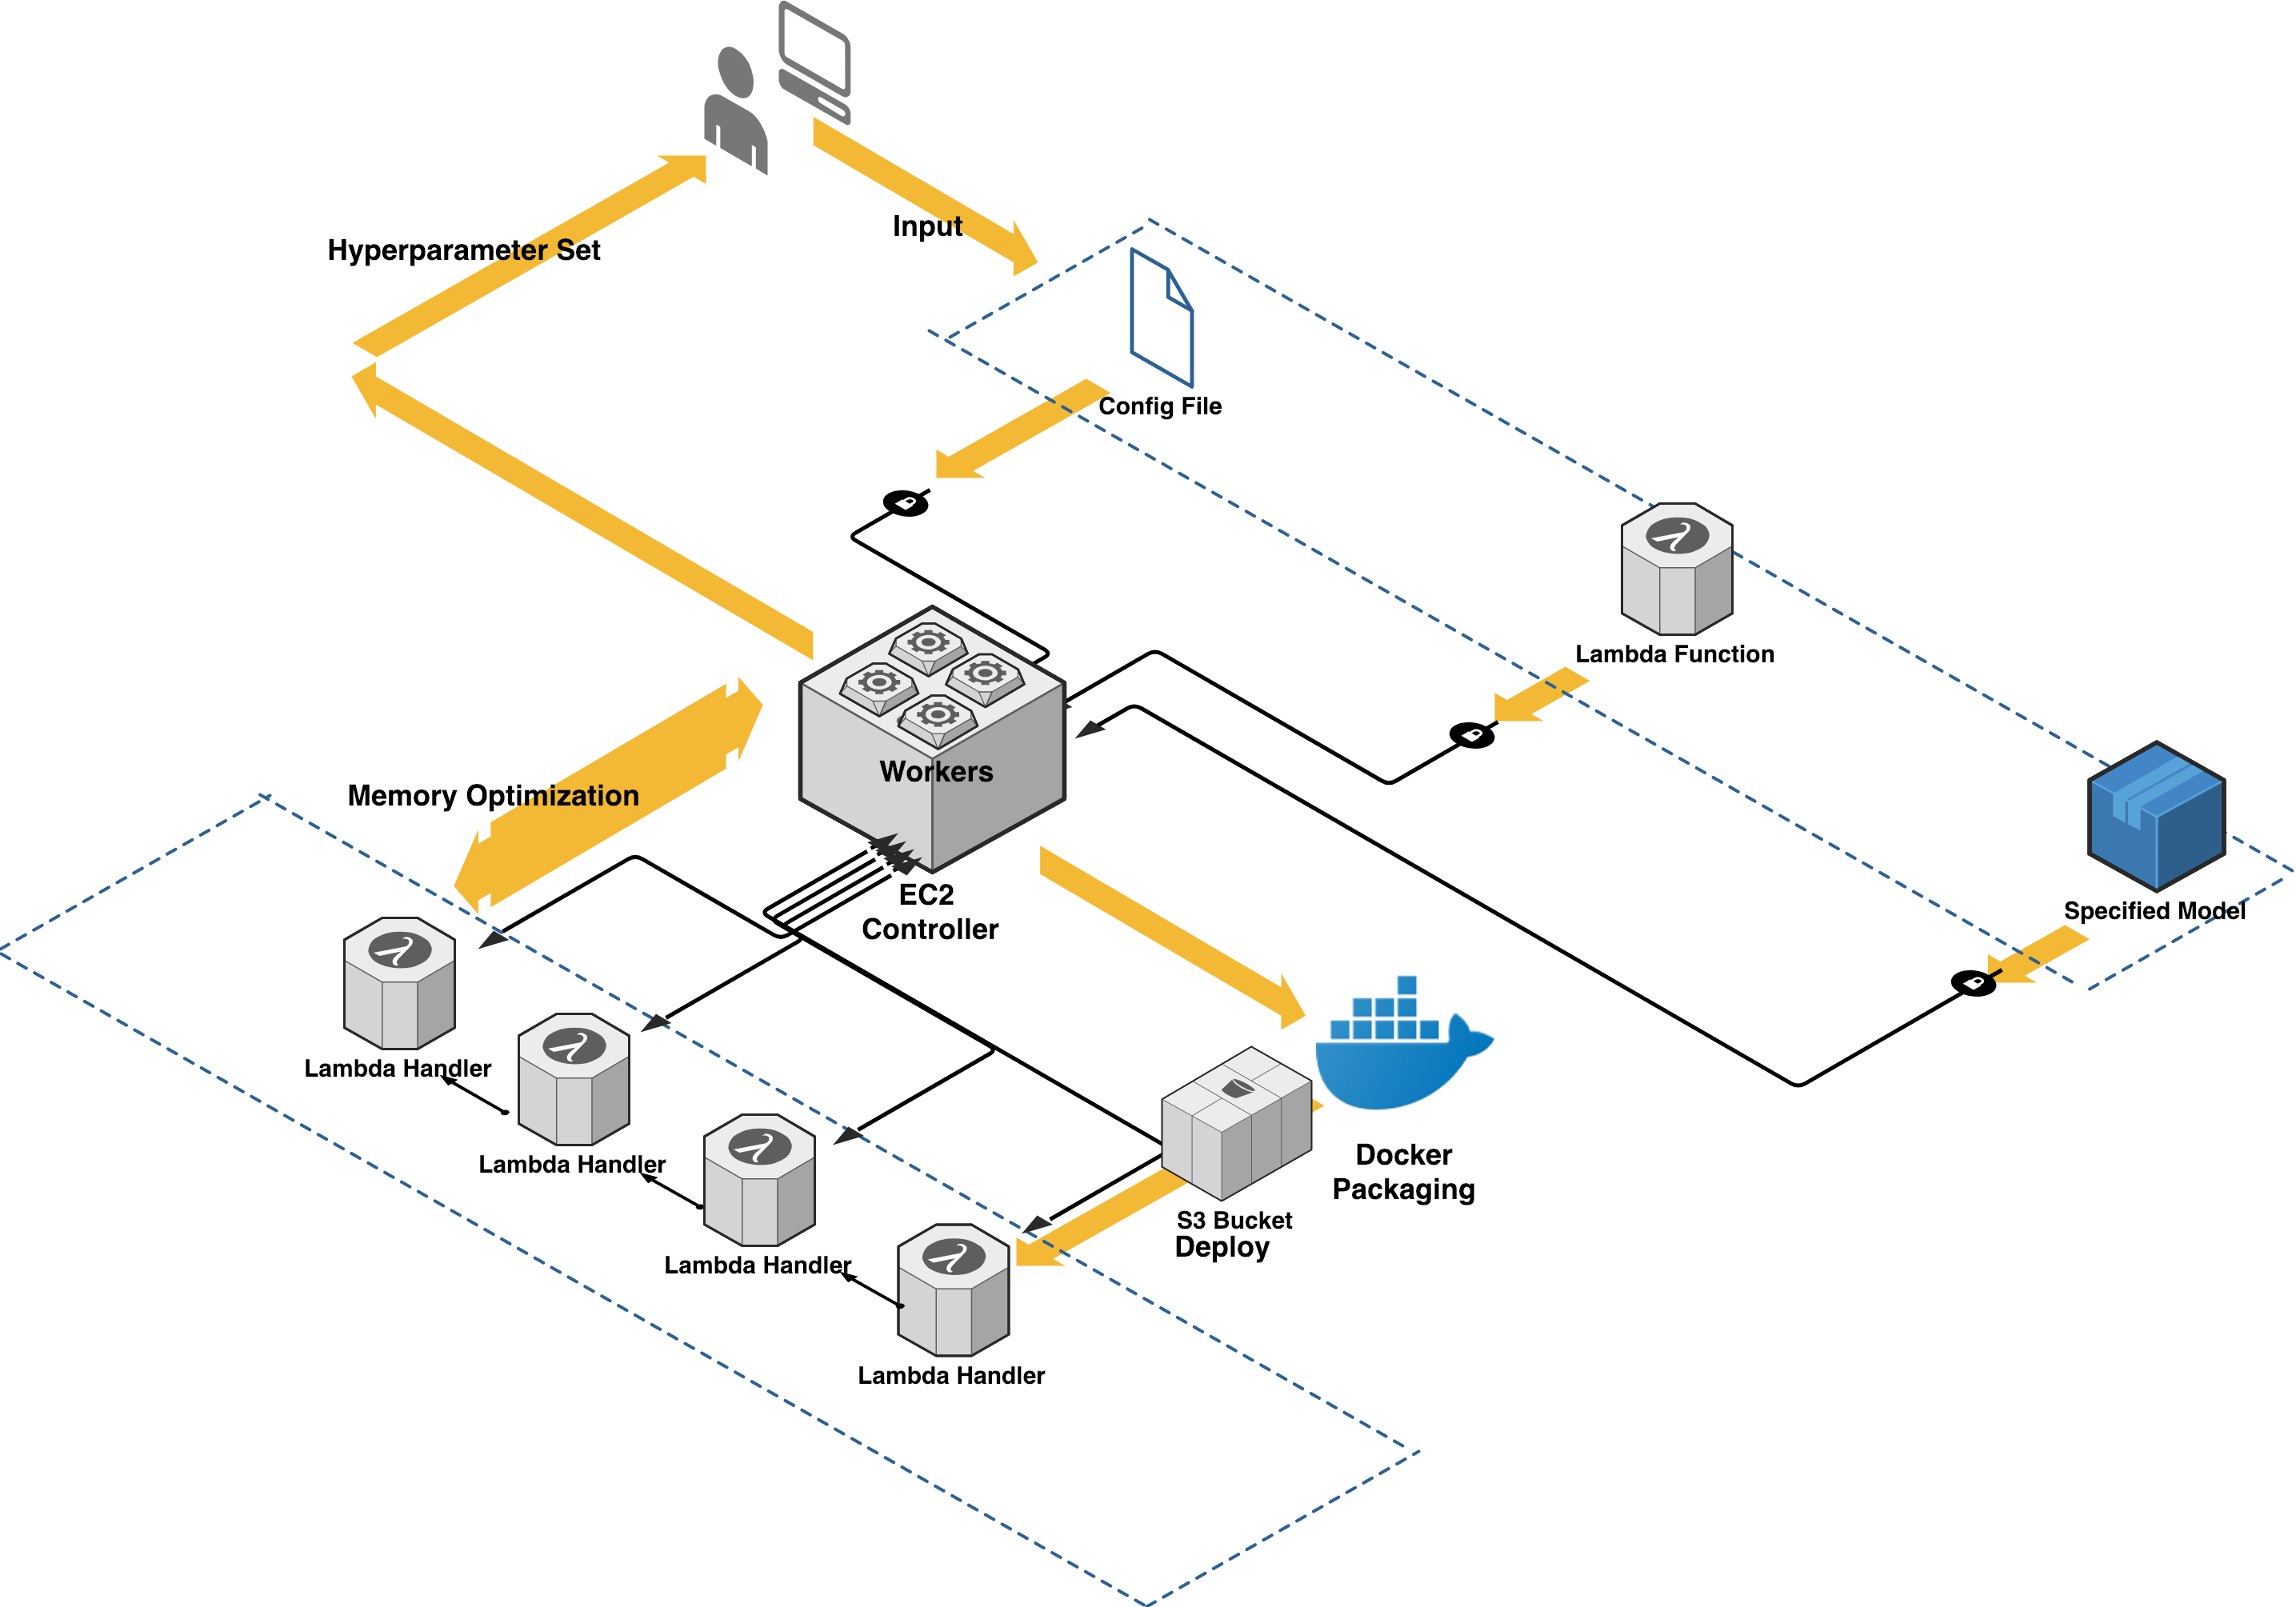
\includegraphics[scale=0.08]{Seneca}
\caption{The architecture of Seneca. 
User specifies hyperparameter options in the configuration file and provides lambda function. Seneca automatically package, deploy and optimize lambda function on AWS before completing grid search process and selecting best hyperparameter setting.
\label{fig:seneca}}
% \vspace{-0.2in}
\end{figure}

To facilitate model search and selection using the serverless architecture, 
we have developed Seneca, 
a framework for tuning the hyperparameters of machine learning applications 
in AWS Lambda. 
The Seneca pipeline consists of packaging, deployment, 
function optimization, and hyperparameter tuning. Figure~\ref{fig:seneca} 
shows the architecture of Seneca.  In the the upper-right-front, we
show the three inputs that Seneca expects from its users: a hyperparameter
configuration file, a dataset URL, and the path to 
the machine learning application.
The configuration file
specifies the range of values for each hyperparameter that the 
application expects.  Seneca uses this configuration to construct
the hyperparameter search space.  The dataset URL refers to a
valid dataset stored in the AWS Simple Storage 
Service (S3)\footnote{\url{https://aws.amazon.com/s3/}}.

Seneca automatically builds and deploys a AWS Lambda application
from the machine learning application specified.
To do so, Seneca launches a docker container that mirrors the
AWS Lambda execution environment, checks and installs
the machine learning application and any libraries it requires,
and compresses the application and uploads it to S3 (avoiding
the AWS Lambda handler size restriction of 10MB).
Seneca constructs an AWS Lambda handler from a template
that, when executed, will download and uncompress the application,
download the dataset and split it into a training and testing set,
and construct, test, and evaluate a model using the application
and a set of hyperparameter values passed in by Seneca as arguments.
Users can specify the train/test split that should be used by Seneca; the
default is 80\%/20\% for classification tasks.
The handler returns a testing score. 
Upon completion of this process, the container deploys the handler
to AWS Lambda using the
AWS Command line Interface\footnote{\url{https://aws.amazon.com/cli/}} 
and the developers credentials.



\subsection{Optimizing Memory Use}

The AWS Lambda pricing model is determined by the execution duration 
and memory of each invoked function. The cost of a function instance is referred to as 
the \texttt{compute charge}, which is the allocated memory 
multiplied by the
billed duration (execution time rounded up to the 
nearest 100ms)~\footnote{\url{https://aws.amazon.com/lambda/pricing/}}.
%https://aws.amazon.com/lambda/pricing/
To ensure that we keep the cost of Seneca as low as possible, we investigate
the impact of this pricing model on application execution and use
our findings to optimize cost.

Currently, allocated memory for a Lambda function can be set
from 128MB to 3008MB in increments of 64MB.
AWS documentation~\footnote{\url{https://docs.aws.amazon.com/lambda/latest/dg/resource-model.html}} 
states that Lambda 
allocates CPU in a way that is proportional to allocated memory size,
as is done for general purpose AWS EC2 instance types.

\begin{figure}[t] \centering 
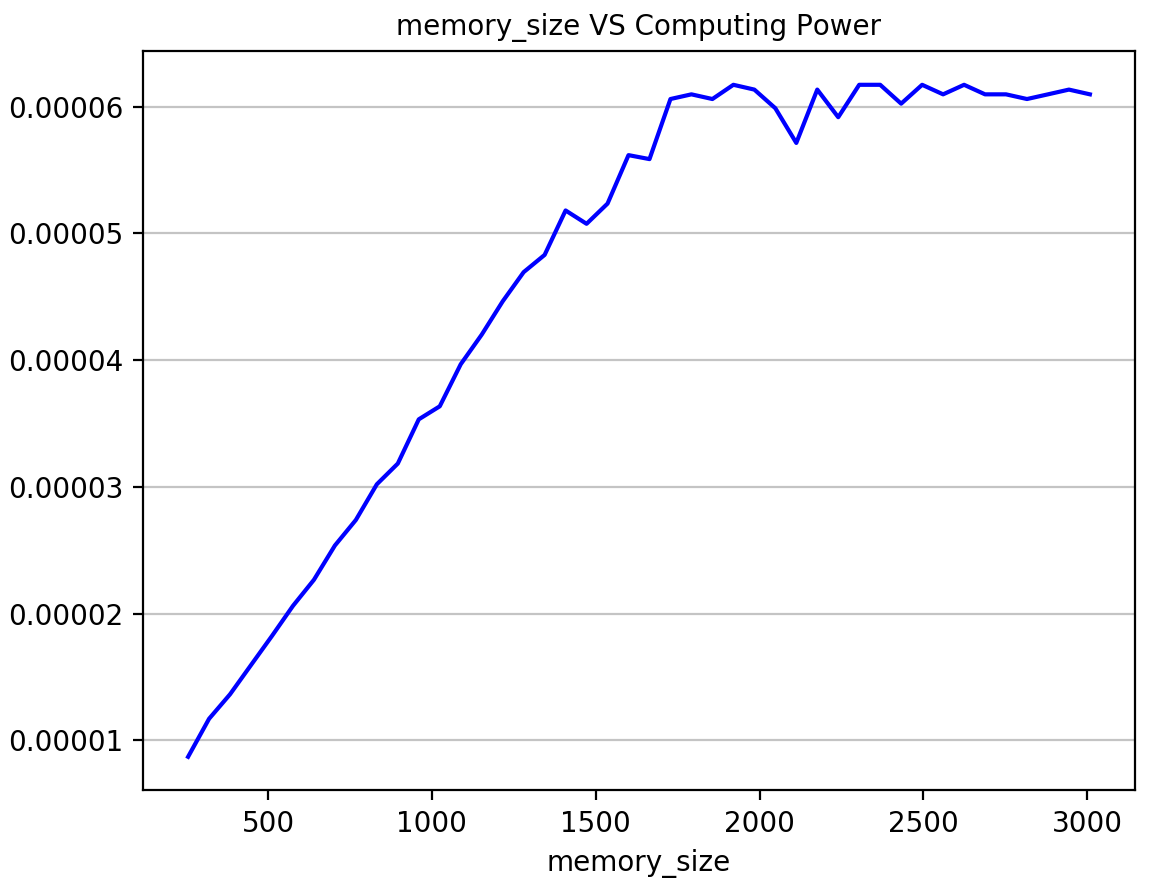
\includegraphics[scale=0.5]{memory}
\caption{The relationship between allocated memory and reciprocal of billed duration, which represents compute power for a compute-bound Lambda function.
\label{fig:memory}}
% \vspace{-0.2in}
\end{figure}

\begin{figure}[t] \centering 
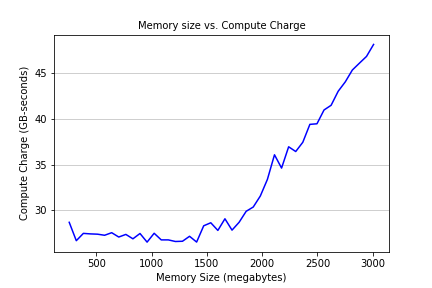
\includegraphics[scale=0.5]{compute_charge}
\caption{The relationship between allocated memory and compute charge for a compute-bound Lambda function.
\label{fig:compute_charge}}
% \vspace{-0.2in}
\end{figure}


To evaluate the impact of memory and CPU allocation on application cost,
we analyze a 3-D matrix multiple serverless benchmark~\cite{ref:matrix} using AWS Lambda.
We configure function instances to use the 46 possible allocated 
memory increments, invoke them, and record the billed duration and memory used by each.
Figure~\ref{fig:memory} shows the relationship between allocated memory 
(x-axis) and reciprocal of billed duration (y-axis). 
Figure~\ref{fig:compute_charge} shows the relationship between memory 
size (x-axis) and compute charge (y-axis). 
We observe that for this benchmark,
the CPU power plateaus after 1600 MB. 
Correspondingly, the compute charge declines from 128 MB to 1600 MB 
and then increases linearly. 

These findings show that CPU does not increase proportionally with
an increase in allocated memory.  We use this relationship within
Seneca to optimize its cost (compute charge) via an extension
that enables it to automatically identify the appropriate
setting for allocated memory for each application.
However, instead of exhaustively testing all 46 possible 
memory configurations, which might be costly,  
Seneca employs the heuristic outlined in
Algorithm~\ref{algo:optimizer}. 

The Seneca optimizer first configures and invokes the function using 
a user-defined payload.  From this run, Seneca obtains the memory 
used by function (reported by AWS Cloudwatch), 
which it uses as its starting point.
Seneca then defines two double-ended queues 
(\texttt{deque}) of length N, to store 
allocated memory and compute charge data of different
invocations. While the current 
allocated memory is less than or equal to 3008 MB, 
the optimizer reconfigures and invokes the function 
using the next increment for memory allocation.  It 
calculates the compute charge for each invocation 
using current allocated memory and billed duration. 

We employ two exit conditions.  The first is when the 
compute charge monotonically increases across \texttt{deque}. 
The second is when the increase in slope is greater than a threshold. 
Once the optimizer finds that both conditions hold, 
it pops the left-most value from \texttt{deque} and configures 
the function to use that value for allocated memory for all future invocations.
After extensive experimentation, we find that 
N=5 and a slope threshold of 1 work well in most cases.
These values can be changed by users of the system however.
In addition, this optimization can be turned on or off via a command line
argument to Seneca.

\begin{algorithm}[]
\SetAlgoLined
\KwData{Typical payload}
\KwResult{Optimal allocated memory}
Find memory used by payload as starting point\;
Define deque for allocated memory \& compute charge\;
 \While{allocated memory $\leq$ 3008 MB}{
  
  \eIf{compute charge monotonically increases in deque \& slope $\geq$ 1}{
   Popleft from deque\;
   Configure allocated memory of function\; 
   Exit\;
   }{
   Increase allocated memory by 64 MB\;
   Probe lambda function\;
   Append allocated memory and compute charge to deque\;
  }
 }
 \caption{Seneca Optimizer Heuristic}
 \label{algo:optimizer}
\end{algorithm}

\subsection{Tuning Process}

For parallel function invocation, Seneca integrates 
Celery~\cite{ref:celery}. Celery is an asynchronous task queue 
that uses distributed message passing. Celery workers are processes 
that take tasks from the queue, execute the tasks with the arguments specified, 
and store the result that is returned 
in a database (we use Redis~\footnote{\url{https://redis.io/}} in our prototype). 

Based on the configuration file, Seneca creates a list of 
payloads (function arguments) with
hyperparameter values.  
The complete list contains all combinations of the specified parameter
settings.  Seneca places the list on the queue and celery 
workers invoke the Lambda handler of the application, passing in the
payload (hyperparameter values) to the handler to use for model construction.  
Upon function
termination, the worker records the evaluation score (and serialized model)
in the database with the hyperparameter configuration from the payload.
When the queue is drained and all workers have completed, Seneca
extracts and reports the best score, configuration, and model from the database.
Users can then evaluate the prediction power of the models (using Seneca if desired) 
for other datasets (to amortize the time/cost of Seneca) without retraining. 

We assume that the dataset supplied to Seneca by the user
is representative of datasets on which the 
resulting model will be used.  In addition, we use prediction error as the 
score (i.e., mean squared error for regression and accuracy percentage for classification) 
instead of $R^2$, which describes explanatory power, to avoid overfitting.
As part of future work, we are considering using multiple datasets and a ranges
of hyperparameter values (versus lists) to preclude the need for users to specify
them and to consider a wider range of values.
